\documentclass[submit]{harvardml}

% Put in your full name and email address.
\name{Your Name}
\email{email@fas.harvard.edu}

% List any people you worked with.
\collaborators{%
  John Doe,
  Fred Doe
}

% You don't need to change these.
\course{CS181-S17}
\assignment{Assignment \#1}
\duedate{5:00pm February 3, 2017}

\usepackage[OT1]{fontenc}
\usepackage[colorlinks,citecolor=blue,urlcolor=blue]{hyperref}
\usepackage[pdftex]{graphicx}
\usepackage{subfig}
\usepackage{fullpage}
\usepackage{amsmath}
\usepackage{amssymb}
\usepackage{color}
\usepackage{todonotes}
\usepackage{listings}
\usepackage{common}

\usepackage[mmddyyyy,hhmmss]{datetime}

\definecolor{verbgray}{gray}{0.9}

\lstnewenvironment{csv}{%
  \lstset{backgroundcolor=\color{verbgray},
  frame=single,
  framerule=0pt,
  basicstyle=\ttfamily,
  columns=fullflexible}}{}
 

\begin{document}
\begin{center}
{\Large Homework 1: Linear Regression}\\
\end{center}



\subsection*{Introduction}
This homework is on different forms of linear regression and focuses
on loss functions, optimizers, and regularization. Linear regression 
will be one of the few models that we see that has an analytical solution.
These problems focus on deriving these solutions and exploring their 
properties. 

If you find that you are having trouble with the first couple
problems, we recommend going over the fundamentals of linear algebra
and matrix calculus. We also encourage you to first read the Bishop
textbook, particularly: Section 2.3 (Properties of Gaussian
Distributions), Section 3.1 (Linear Basis Regression), and Section 3.3
(Bayesian Linear Regression). (Note that our notation is slightly different but
the underlying mathematics remains the same :).

Please type your solutions after the corresponding problems using this \LaTeX\ template, and start each problem on a new page.\\

\pagebreak 

%%%%%%%%%%%%%%%%%%%%%%%%%%%%%%%%%%%%%%%%%%%%%
% Problem 1
%%%%%%%%%%%%%%%%%%%%%%%%%%%%%%%%%%%%%%%%%%%%%
\begin{problem}[Centering and Ridge Regression, 7pts]

  Consider a data set $D = \{(\boldx_i, y_i)\}_{i=1}^n$ in which each
  input vector $\boldx \in \mathbb{R}^m$. As we saw in lecture, this
  data set can be written using the design matrix $\boldX \in
  \mathbb{R}^{n \times m}$ and the target vector $\boldy \in \reals^n$.
  
  
  For this problem assume that the input matrix is centered, that is
  the data has been pre-processed such that $\frac{1}{n} \sum_{i=1}^n
  x_{ij} = 0 $.  Additionally we will use a positive regularization
  constant $\lambda > 0$ to add a ridge regression term.

  In particular we consider a ridge regression loss function of the following form,

\[\mcL(\boldw, w_0) = (\boldy - \boldX \boldw - w_0 {\bf 1 })^\top (\boldy - \boldX
\boldw - w_0 {\bf 1 }) + \lambda \boldw^\top \boldw .\]

 Note that we are not incorporating the bias $w_0\in \reals$ into the weight parameter $\boldw \in \reals^m$.
 For this problem the notation ${\bf 1}$ indicates a vector of all 1's, in this case in implied to be in $\reals^n$.  


\begin{itemize}
  \item[(a)] Compute the gradient of $\mcL(\boldw, w_0)$ with respect to $w_0$.
    Simplify as much as you can for full credit.
  \item[(b)] Compute the gradient of $\mcL(\boldw, w_0)$ with respect to $\boldw$.
    Simplify as much as you can for full credit. Make sure to give your answer
    in vector form.
  \item[(c)] Suppose that $\lambda > 0$. Knowing that $\mcL$ is a convex function
    of its arguments, conclude that a global optimizer of
    $\mcL(\boldw, w_0)$ is
    \begin{align}
      w_0 &= \frac{1}{n} \sum_{i=1}^n y_i \\
      \boldw &= (\boldX^\top \boldX + \lambda \boldI)^{-1} \boldX^\top \boldy
    \end{align}
  \item[(d)] In order to take the inverse in the previous question, the
    matrix $(\boldX^\top \boldX + \lambda \boldI)$ must be invertible.
    One way to ensure invertibility is by showing that a matrix is
    \textit{positive definite}, i.e. it has all positive
    eigenvalues. Given that $\boldX^\top\boldX$ is positive
    \textit{semi}-definite, i.e.  all non-negative eigenvalues, prove that the
    full matrix is invertible.

  \item[(e)] What difference does the last problem highlight standard least-squares regression versus
    ridge regression?

\end{itemize}
\end{problem}

\subsubsection*{Solution}











%%%%%%%%%%%%%%%%%%%%%%%%%%%%%%%%%%%%%%%%%%%%%
% Problem 2
%%%%%%%%%%%%%%%%%%%%%%%%%%%%%%%%%%%%%%%%%%%%%
\newpage
%\subsection*{2. Priors and Regularization [7pts]}
\begin{problem}[Priors and Regularization,7pts]
In this problem we consider a model of Bayesian linear regression. Define the prior on the parameters as,
\begin{align*}
p(\boldw) = \mathcal{N}(\boldw \given \bold0, \alpha^{-1}\ident ),
\end{align*}
where $\alpha$ is as scalar precision hyperparameter that controls the variance of the Gaussian prior.  Define the likelihood as,
\begin{align*}
p(\boldy \given \boldx) &= \prod_{i=1}^n \mcN(y_i \given \boldw^\trans \boldx_i, \beta^{-1}),
\end{align*}
where $\beta$ is another fixed scalar defining the variance. \\


\noindent Using the fact that the posterior is the product of the prior and the likelihood (up to a normalization constant), i.e., 
\[\arg\max_{\boldw} \ln p(\boldw \given \boldy)= \arg\max_{\boldw} \ln p(\boldw) + \ln p(\boldy \given \boldw).\]

\noindent Show that maximizing the log posterior is equivalent to minimizing a regularized loss function given by ${\mcL(\boldw) + \lambda \mcR(\boldw)}$, where
\begin{align*}
\mcL(\boldw) &= \frac{1}{2}\sum_{i = 1}^n (y_i - \boldw^\trans \boldx_i)^2 \\
\mcR(\boldw) &= \frac{1}{2}\boldw^\trans \boldw
\end{align*} \\

\noindent Do this by writing $\ln p(\boldw \given \boldy)$ as a function of $\mcL(\boldw)$ and $\mcR(\boldw)$, dropping constant terms if necessary.  Conclude that maximizing this posterior is equivalent to minimizing the regularized error term given by $\mcL(\boldw) + \lambda \mcR(\boldw)$ for a $\lambda$ expressed in terms of the problem's constants.  
\end{problem}


\subsubsection*{Solution}



























%%%%%%%%%%%%%%%%%%%%%%%%%%%%%%%%%%%%%%%%%%%%%
% Problem 3
%%%%%%%%%%%%%%%%%%%%%%%%%%%%%%%%%%%%%%%%%%%%%
\newpage
\subsection*{3. Modeling Changes in Congress [10pts]}
 The objective of this problem is to learn about linear regression with basis
 functions by modeling the average age of the US Congress. The file
 \verb|congress-ages.csv| contains the data you will use for this problem.  It
 has two columns.  The first one is an integer that indicates the Congress
 number. Currently, the 114th Congress is in session. The second is the average
 age of that members of that Congress.  The data file looks like this:
\begin{csv}
congress,average_age
80,52.4959
81,52.6415
82,53.2328
83,53.1657
84,53.4142
85,54.1689
86,53.1581
87,53.5886
\end{csv}
and you can see a plot of the data in Figure~\ref{fig:congress}.

\begin{figure}[h]
\centering
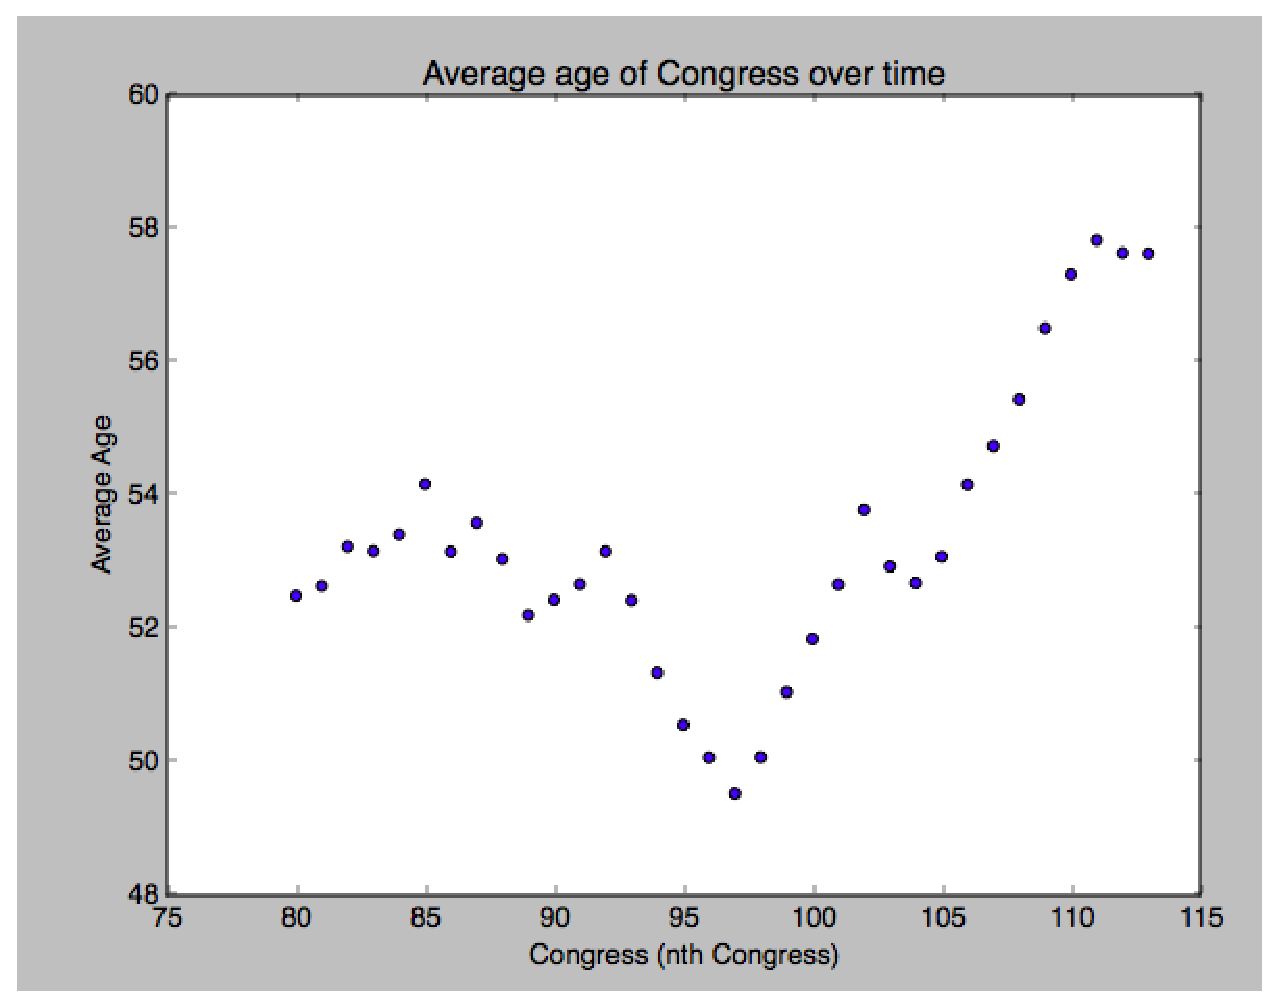
\includegraphics[width=0.8\textwidth]{congress-ages}
\caption{Average age of Congress.  The horizontal axis is the Congress number, and the vertical axis is the average age of the congressmen.}
\label{fig:congress}
\end{figure}

\begin{problem}[Modeling Changes in Congress, 10pts]
Implement basis function regression with ordinary least squares with the above
data. Some sample Python code is provided in \verb|linreg.py|, which implements
linear regression.  Plot the data and regression lines for the simple linear
case, and for each of the following sets of basis functions:
\begin{itemize}
	\item[(a)] $\phi_j(x) = x^j$ for $j=1, \ldots, 6$
	\item[(b)] $\phi_j(x) = x^j$ for $j=1, \ldots, 4$
	\item[(c)] $\phi_j(x) = \sin(x / j)$ for $j=1, \ldots, 6$
	\item[(d)] $\phi_j(x) = \sin(x / j)$ for $j=1, \ldots, 10$
	\item[(e)] $\phi_j(x) = \sin(x / j)$ for $j=1, \ldots, 22$
\end{itemize}
  In addition to the plots, provide one or two sentences for each, explaining
  whether you think it is fitting well, overfitting or underfitting.  If it does
  not fit well, provide a sentence explaining why. A good fit should capture the
  most important trends in the data.
	\end{problem}

\subsubsection*{Solution}











\newpage
\begin{problem}[Calibration, 1pt]
Approximately how long did this homework take you to complete?
\end{problem}
\textbf{Answer:}

\end{document}
